%%%%(c)
%%%%(c)  This file is a portion of the source for the textbook
%%%%(c)
%%%%(c)    Abstract Algebra: Theory and Applications
%%%%(c)    Copyright 1997 by Thomas W. Judson
%%%%(c)
%%%%(c)  See the file COPYING.txt for copying conditions
%%%%(c)
%%%%(c)
\chap{Rings}{rings}
 
Up to this point we have studied sets with a single binary operation
satisfying certain axioms, but often we are more interested in working
with sets that have two binary operations.  For example, one of the
most natural algebraic structures to study is the integers 
with the operations of addition and multiplication. These operations
are related to one another by the distributive
property. If we consider a set with two such related binary operations
satisfying certain axioms, we have an algebraic structure called a
ring. In a ring we add and multiply such elements as real numbers,
complex numbers, matrices, and functions. 
 

\section{Rings}

A nonempty set $R$ is a {\bfi ring\/}\index{Ring!definition of} if
it has two closed binary operations, addition and multiplication,
satisfying the following conditions.  
\begin{enumerate}
 
\item
$a + b = b + a$ for $a, b \in R$.
 
\item
$(a + b) + c = a + ( b + c)$ for $a, b, c  \in R$.
 
\item
There is an element $0$ in $R$ such that $a + 0 = a$ for all $a \in
R$. 
 
\item
For every element $a \in R$, there exists an element $-a$ in $R$ such
that $a + (-a) = 0$. 
 
\item
$(ab)  c = a  ( b  c)$ for $a, b, c  \in R$.
 
\item
For $a, b, c \in R$,
\begin{align*}
a( b + c)&  = & ab +ac \\
(a + b)c & = ac + bc.
\end{align*}
 
\end{enumerate}
This last condition, the distributive axiom, relates the binary
operations of addition and multiplication. Notice that the first four
axioms simply require that a ring be an abelian group under addition,
so we could also have defined a ring to be an abelian group
$(R, +)$ together with a second binary operation satisfying the fifth
and sixth conditions given above.  
 
 
If there is an element $1 \in R$ such that $1 \neq 0$ and  $1a = a1 =
a$ for each element $a \in R$, we say that $R$ is a ring with {\bfi
unity\/}\index{Ring!with unity} or {\bfi identity\/}\index{Ring!with
identity}. A ring $R$ for which $ab = ba$ for all $a, 
b$ in $R$ is called a {\bfi commutative
ring}\index{Ring!commutative}\index{Commutative rings}. A commutative
ring $R$ with identity is called an {\bfi integral
domain\/}\index{Integral domain} if, for every $a, b  \in R$ such that
$ab = 0$, either $a = 0$ or $b = 0$.  A {\bfi division
ring\/}\index{Division ring}\index{Ring!division} is a ring $R$, with an
identity, in which every nonzero element in $R$ is a {\bfi
unit}\index{Unit}; that is, for each $a \in R$ with $a \neq 0$, there
exists a unique element $a^{-1}$ such that $a^{-1} a = a a^{-1}  = 1$.
A commutative division ring is called a {\bfi field}\index{Field}. 
The relationship among rings, integral domains, division rings, and
fields is shown in Figure~\ref{Rings}.  
 
\begin{figure}[hbt] %Replaced figure with tikz figure - TWJ 8/13/2010
\begin{center}
\tikzpreface{rings_types}
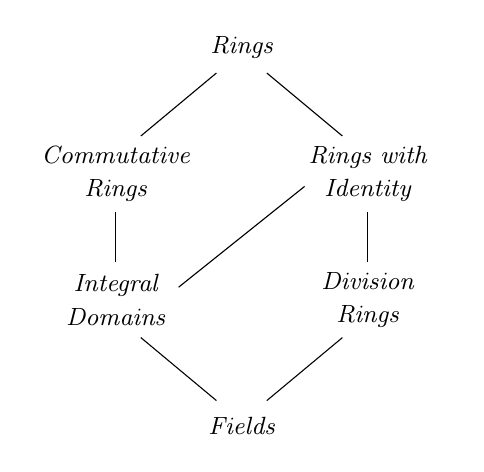
\begin{tikzpicture}[scale=0.8]

\draw  (2,0.4) -- (2,-0.4);
\draw  (-2,0.4) -- (-2,-0.4);
\draw  (1,0.8) -- (-1,-0.8);
\draw  (1.6,1.6) -- (0.4,2.6);
\draw  (-1.6,1.6) -- (-0.4,2.6);
\draw  (1.6,-1.6) -- (0.4,-2.6);
\draw  (-1.6,-1.6) -- (-0.4,-2.6);

\node [text width=2cm, text centered] at (2, 1) {\small \it Rings with Identity};
\node [text width=1.5cm, text centered] at (2, -1) {\small \it Division Rings};

\node [text width=2cm, text centered] at (-2, 1) {\small \it Commutative Rings};
\node [text width=1.5cm, text centered] at (-2, -1) {\small \it Integral Domains};

\node at (0,3) {\small \it Rings};
\node at (0,-3) {\small \it Fields};
\end{tikzpicture}

\end{center}
\caption{Types of rings}
\label{Rings}
\end{figure}
 
 
 
\begin{example}{integer_ring}
As we have mentioned previously, the integers form a ring. In fact, ${\mathbb
Z}$ is an integral domain.  Certainly if $a b = 0$ for two integers
$a$ and $b$, either $a=0$ or $b=0$. However, ${\mathbb Z}$ is not a
field. There is no integer that is the multiplicative inverse of 2,
since $1/2$ is not an integer.  The only integers with multiplicative
inverses are 1 and $-1$.  
\end{example}
 
 
\begin{example}{field_ring}
Under the ordinary operations of addition and multiplication, all of
the familiar number systems are rings: the rationals, ${\mathbb Q}$; the
real numbers, ${\mathbb R}$; and the complex numbers, ${\mathbb C}$. Each of
these rings is a field. 
\end{example}
 
 
\begin{example}{Zn_rings}
We can define the product of two elements $a$ and $b$ in ${\mathbb Z}_n$
by $ab~\pmod{n}$. For instance, in ${\mathbb Z}_{12}$,  $5 \cdot 7 \equiv
11 \pmod{12}$.  This product makes the abelian group ${\mathbb Z}_n$ into
a ring. Certainly ${\mathbb Z}_n$ is a commutative ring; however, it may
fail to be an integral domain.  If we consider $3 \cdot 4 \equiv 0
\pmod{12}$ in ${\mathbb Z}_{12}$, it is easy to see that a product of two 
nonzero elements in the ring can be equal to zero.  
\end{example}

 
 
A nonzero element $a$ in a ring $R$ is called a {\bfi zero
divisor\/}\index{Zero divisor} if there is a nonzero element $b$ in $R$
such that $ab = 0$. In the previous example,  3 and 4 are zero
divisors in ${\mathbb Z}_{12}$.  
 
 
\begin{example}{function_ring}
In calculus the continuous real-valued functions on an interval
$[a,b]$ form a commutative ring. We add or multiply two functions by 
adding or multiplying the values of the functions.  If $f(x) = x^2$ and
$g(x) = \cos x$, then $(f+g)(x) = f(x) + g(x) = x^2 + \cos x$ and
$(fg)(x) = f(x) g(x) = x^2 \cos x$.
\mbox{\hspace{1in}}
\end{example}
 
 
\begin{example}{matrix_ring}
The $2 \times 2$ matrices  with entries in ${\mathbb R}$ form a ring
under the usual operations of matrix addition and multiplication. This
ring is \mbox{noncommutative}, since it is usually the case that $AB \neq
BA$. Also, notice that we can have $AB = 0$ when neither $A$ nor $B$
is zero. 
\end{example}
 
 
\begin{example}{noncommute_ring}
For an example of a noncommutative division ring, let
\[
1 = 
\begin{pmatrix}
1 & 0 \\
0 & 1
\end{pmatrix},
\quad
{\mathbf i}
=
\begin{pmatrix}
0 & 1 \\
-1 & 0
\end{pmatrix},
\quad
{\mathbf j} =
\begin{pmatrix}
0 & i \\
i & 0
\end{pmatrix},
\quad
{\mathbf k} = 
\begin{pmatrix}
i & 0 \\
0 & -i
\end{pmatrix},
\]
where $i^2 = -1$. These elements satisfy the following relations: 
\begin{align*}
{\mathbf i}^2 = {\mathbf j}^2 & =  {\mathbf k}^2 = -1 \\
{\mathbf i}  {\mathbf j} & =  {\mathbf k}  \\
{\mathbf j}  {\mathbf k} & =  {\mathbf i}  \\
{\mathbf k}  {\mathbf i} & =  {\mathbf j}  \\
{\mathbf j}  {\mathbf i} & =  - {\mathbf k}  \\
{\mathbf k}  {\mathbf j} & =  - {\mathbf i}  \\
{\mathbf i}  {\mathbf k} & =  - {\mathbf j}. 
\end{align*}
Let ${\mathbb H}$\label{noteringH} consist of elements of the form $a + b
{\mathbf i}  + c {\mathbf j} +d {\mathbf k}$, where $a, b , c, d$ are real
numbers. Equivalently, ${\mathbb H}$ can be considered to be the set of
all $2 \times 2$ matrices of the form  
\[
\begin{pmatrix}
\alpha & \beta \\
-\overline{\beta} & \overline{\alpha }
\end{pmatrix},
\]
where $\alpha = a + di$ and $\beta = b+ci$ are complex numbers. We can
define addition and multiplication on ${\mathbb H}$ either by the usual matrix
operations or in terms of the generators 1, ${\mathbf i}$, ${\mathbf j}$,
and ${\mathbf k}$: 
\begin{multline*}
(a_1 + b_1 {\mathbf i}  + c_1 {\mathbf j} +d_1 {\mathbf k} )
+ ( a_2 + b_2 {\mathbf i}  + c_2 {\mathbf j} +d_2 {\mathbf k} ) \\
=
(a_1 + a_2) + ( b_1 + b_2) {\mathbf i}  + ( c_1 + c_2)
{\mathbf j} + ( d_1 + d_2) {\mathbf k}
\end{multline*}
and
\[
(a_1 + b_1 {\mathbf i}  + c_1 {\mathbf j} +d_1 {\mathbf k} ) ( a_2 + b_2
{\mathbf i}  + c_2 {\mathbf j} +d_2 {\mathbf k} ) = \alpha + \beta {\mathbf
i}  + \gamma {\mathbf j} + \delta {\mathbf k},
\]
where
\begin{align*}
\alpha & =  a_1 a_2 - b_1 b_2 - c_1 c_2 -d_1 d_2 \\
\beta & =  a_1 b_2 + a_1 b_1 + c_1 d_2 - d_1 c_2 \\
\gamma & =  a_1 c_2 - b_1 d_2 + c_1 a_2 - d_1 b_2 \\
\delta & =  a_1 d_2 + b_1 c_2 - c_1 b_2 - d_1 a_2.
\end{align*}
Though multiplication looks complicated, it is actually a
straightforward computation if we remember that we just add and
multiply elements in ${\mathbb H}$ like polynomials and keep in mind the
relationships between the generators ${\mathbf i}$, ${\mathbf j}$, and
${\mathbf k}$. The ring ${\mathbb H}$ is called the ring of {\bfi
quaternions}\index{Quaternions}.
 
 
To show that the quaternions are a division ring, we must be able to
find an inverse for each nonzero element. Notice that 
\[
( a + b {\mathbf i}  + c {\mathbf j} +d {\mathbf k} )( a - b
{\mathbf i}  - c {\mathbf j}
-d {\mathbf k} ) = a^2 + b^2 + c^2 + d^2.
\]
This element can be zero only if $a$, $b$, $c$, and $d$ are
all zero. So if $a + b {\mathbf i}  + c {\mathbf j} +d {\mathbf k}
\neq 0$,
\[
( a + b {\mathbf i}  + c {\mathbf j} +d {\mathbf k} )
\left(
\frac{a - b {\mathbf i} - c {\mathbf j} - d {\mathbf k} }{ a^2 + b^2 + c^2
+ d^2 }
\right)
= 1.
\]
\end{example}
 
 
\begin{proposition}
Let $R$ be a ring with $a, b \in R$. Then
\begin{enumerate}
 
\rm \item \it
$a0 = 0a = 0$;
 
\rm \item \it
$a(-b) = (-a)b = -ab$;
 
\rm \item \it
$(-a)(-b) =ab$.
 
\end{enumerate}
\end{proposition}
 
 
\begin{proof}
To prove (1), observe that
\[
a0 = a(0+0)= a0+ a0;
\]
hence, $a0=0$. Similarly, $0a = 0$. For (2), we have $ab + a(-b) =
a(b-b) = a0 = 0$; consequently, $-ab = a(-b)$. Similarly, $-ab =
(-a)b$. Part (3) follows directly from (2) since $(-a)(-b) = -(a(- b))
= -(-ab) = ab$. 
\end{proof}
 
 
\medskip
 
 
Just as we have subgroups of groups, we have an analogous class of 
\mbox{substructures} for rings. A {\bfi subring}\index{Subring} $S$ 
of a ring
$R$ is a subset $S$ of $R$ such that $S$ is also a ring under the
inherited operations from $R$.
 
 
\begin{example}{subring_chain}
The ring $n {\mathbb Z}$ is a subring of ${\mathbb Z}$.  Notice that even
though the original ring may have an identity, we do not require
that its subring have an identity. We have the following chain of
subrings: 
\[
{\mathbb Z} \subset {\mathbb Q} \subset {\mathbb R} \subset {\mathbb C}.
\]
\end{example}
 
 

 
 
The following proposition gives us some easy criteria for determining
whether or not a  subset of a ring is indeed a subring. (We will leave
the proof of this proposition as an exercise.)
 
 
\begin{proposition}
Let $R$ be a ring and $S$ a subset of $R$.  Then $S$ is a subring of
$R$ if and only if the following conditions are satisfied. 
\begin{enumerate}
 
\rm \item \it
$S \neq \emptyset$.
 
\rm \item \it
$rs \in S$ for all $r, s \in S$.
 
\rm \item \it
$r-s \in S$ for all $r, s \in S$.
 
\end{enumerate}
\end{proposition}
 
 
\begin{example}{M2_ring}
Let  $R ={\mathbb M}_2( {\mathbb R} )$ be the ring of $2 \times 2$ matrices
with entries in ${\mathbb R}$. If $T$ is the set of upper triangular
matrices in $R$; i.e.,
\[
T =
\left\{
\begin{pmatrix}
a & b \\
0 & c
\end{pmatrix}
: a, b, c \in {\mathbb R}
\right\},
\]
then $T$ is a subring of $R$. If
\[
A=
\begin{pmatrix}
a & b \\
0 & c
\end{pmatrix}
\quad \text{and} \quad
B =
\begin{pmatrix}
a' & b' \\
0 & c'
\end{pmatrix}
\]
are in $T$, then clearly $A-B$ is also in $T$. Also,
\[
AB =
\begin{pmatrix}
a a' & ab' + bc' \\
0 & cc'
\end{pmatrix}
\]
is in $T$.
\end{example}
 
 
 
\section{Integral Domains and Fields}
 
 
Let us briefly recall some definitions. If $R$ is a ring and $r$ is a
nonzero element in $R$, then $r$ is said to  be a {\bfi zero divisor\/}
if there is some nonzero element $s \in R$ such that $rs = 0$. A
commutative ring with identity is said to be an {\bfi integral
domain\/} if it has no zero divisors.  If an element $a$ in a ring $R$
with identity has a multiplicative inverse, we say that $a$ is a {\bfi
unit}. If every nonzero element in a ring $R$ is a unit, then $R$ is
called a {\bfi division ring}.  A commutative division ring is called
a {\bfi field}. 
 
 
\begin{example}{gaussian_ring}
If $i^2 = -1$, then the set ${\mathbb Z}[ i ] = \{ m + ni : m, n \in
{\mathbb Z} \}$ forms a ring known as the {\bfi Gaussian
integers}\index{Gaussian integers}\label{gaussianintegers}. It is
easily seen that the Gaussian integers are a subring of the complex
numbers since they are closed under addition and multiplication. Let
$\alpha = a + bi$ be a unit in ${\mathbb Z}[ i ]$. Then
$\overline{\alpha} = a - bi$ is also a unit since if $\alpha \beta =
1$, then $\overline{\alpha} \overline{\beta} = 1$. If $\beta = c +
di$, then   
\[
1 = \alpha \beta \overline{\alpha} \overline{\beta} = (a^2 +
b^2 )(c^2
+ d^2).
\]
Therefore, $a^2 + b^2$ must either be 1 or $-1$; or, equivalently, $a
+ bi = \pm 1$ or $a+ bi = \pm i$.  Therefore, units of this ring are
$\pm 1$ and $\pm i$; hence, the Gaussian integers are not a field. We
will leave it as an exercise to prove that the Gaussian integers are
an integral domain. 
\end{example}
 
 
\begin{example}{matrix_Z2}
The set of matrices
\[
F
=
\left\{
\begin{pmatrix}
1 & 0 \\
0 & 1
\end{pmatrix},
\begin{pmatrix}
1 & 1 \\
1 & 0
\end{pmatrix},
\begin{pmatrix}
0 & 1 \\
1 & 1
\end{pmatrix},
\begin{pmatrix}
0 & 0 \\
0 & 0
\end{pmatrix}
\right\}
\]
with entries in ${\mathbb Z}_2$ forms a field.
\end{example}
 
 
\begin{example}{Q_sqrt2_field}
The set ${\mathbb Q}( \sqrt{2}\, ) = \{ a + b \sqrt{2} : a, b \in {\mathbb Q}
\}$ is a field. The inverse of an element $a + b \sqrt{2}$ in ${\mathbb
Q}( \sqrt{2}\, )$ is  
\[
\frac{a}{a^2 - 2 b^2} +\frac{- b}{ a^2 - 2 b^2} \sqrt{2}.
\]
\end{example}
 
 

 
 
We have the following alternative characterization of integral
domains. 
 
 

 
 
\begin{proposition}[Cancellation Law]\index{Cancellation law!for
integral domains}
Let $D$ be a commutative ring with identity. Then $D$ is an integral
domain if and only if for all nonzero elements $a \in D$ with $ab =
ac$, we have $b=c$. 
\end{proposition}
 
 
\begin{proof}
Let $D$ be an integral domain. Then $D$ has no zero divisors.  Let $ab
= ac$ with $a \neq 0$. Then $a(b - c) =0$.  Hence, $b - c = 0$ and $b
= c$. 
 
 
Conversely, let us suppose that cancellation is possible in $D$.
That is, suppose that $ab = ac$ implies $b=c$. Let $ab = 0$.  If $a
\neq 0$, then $ab = a 0$ or $b=0$.  Therefore, $a$ cannot be a zero
divisor. 
\end{proof}
 
 
\medskip
 
 
The following surprising theorem is due to Wedderburn.
 
 
\begin{theorem}
Every finite integral domain is a field.
\end{theorem}
 
 
\begin{proof}
Let $D$ be a finite integral domain and $D^\ast$ be the set of nonzero
elements of $D$.  We must show that every element in $D^*$ has an
inverse. For each $a \in D^\ast$ we can define a map $\lambda_a :
D^\ast \rightarrow D^\ast$ by $\lambda_a(d) = ad$.  This map makes
sense, because if  $a \neq 0$ and $d \neq 0$, then $ad \neq 0$.  The map
$\lambda_a$ is one-to-one, since for $d_1, d_2 \in D^*$, 
\[
ad_1 = \lambda_a(d_1) = \lambda_a(d_2) = ad_2
\]
implies $d_1 = d_2$ by left cancellation. Since $D^\ast$ is a finite
set, the map $\lambda_a$ must also be onto; hence, for some $d \in
D^\ast$, $\lambda_a(d) = ad = 1$. Therefore, $a$ has a left inverse.
Since $D$ is commutative, $d$ must also be a right inverse for $a$.
Consequently, $D$ is a field. 
\end{proof}
 
 
\medskip
 
 
For any nonnegative integer $n$ and any element $r$ in a ring $R$ we 
write $r + \cdots + r$ ($n$ times) as $nr$. We  define the {\bfi
characteristic\/}\index{Characteristic of a
ring}\index{Ring!characteristic of}\label{ringchar} of a ring $R$ to 
be the least positive integer $n$ such that $nr=0$ for all $r \in R$.
If no such integer exists, then the characteristic of $R$ is defined
to be 0.  
 
 
\begin{example}{Zp_field}
For every prime $p$, ${\mathbb Z}_p$ is a field of characteristic $p$. By
Proposition~\ref{Zn_equiv_classes}, every nonzero element in ${\mathbb Z}_p$ has an inverse;
hence, ${\mathbb Z}_p$ is a field. If $a$ is any nonzero element in the
field, then $pa =0$, since the order of any nonzero element in the
abelian group ${\mathbb Z}_p$ is $p$. 
\end{example}
 
 
\begin{theorem}\label{rings:characteristic_theorem}
The characteristic of an integral domain is either prime or~zero.
\end{theorem}
 
 
\begin{proof}
Let $D$ be an integral domain and suppose that the characteristic of
$D$ is $n$ with $n \neq 0$. If $n$ is not prime, then $n = ab$, where
$1 < a <n$ and $1 < b < n$. Since $0 = n 1 = (ab)1 = (a1)(b1)$ and
there are no zero divisors in $D$, either $a1 =0$ or $b1=0$. Hence,
the characteristic of $D$ must be less than $n$, which is a
contradiction.  Therefore, $n$ must be prime. 
\end{proof}
 
 
 
\section{Ring Homomorphisms and Ideals}
 
 
In the study of groups, a homomorphism is a map that preserves the
operation of the group.  Similarly, a homomorphism between rings
preserves the operations of addition and multiplication in the ring.
More specifically, if  $R$ and $S$ are rings, then   a {\bfi ring
homomorphism\/}\index{Homomorphism!ring}\index{Ring!homomorphism} is a
map $\phi : R \rightarrow S$ satisfying  
\begin{align*}
\phi( a + b ) & = \phi( a ) + \phi(b) \\
\phi( a b ) & = \phi( a ) \phi(b)
\end{align*}
for all $a, b \in R$.  
If $\phi : R \rightarrow S$ is a one-to-one and onto homomorphism,
then $\phi$ is called an {\bfi
isomorphism\/}\index{Isomorphism!ring}\index{Ring!isomorphism} of rings.   
 
 
The set of elements that a ring homomorphism maps to $0$ plays a
fundamental role in the theory of rings. For any ring homomorphism
$\phi : R \rightarrow S$, we define the {\bfi
kernel\/}\index{Homomorphism!kernel of a ring}\index{Kernel!of a ring
homomorphism} of a ring homomorphism to be the set
\[
\ker \phi = \{ r \in R : \phi( r ) = 0 \}.
\]
 
 
\begin{example}{ring_homo}
For any integer $n$ we can define a ring homomorphism $\phi~:~{\mathbb Z}
\rightarrow {\mathbb Z}_n$ by $a \mapsto a \pmod{n}$. This is indeed a
ring homomorphism, since 
\begin{align*}
\phi( a + b )  & = (a + b) \pmod{n} \\
 & =  a \pmod{n} + b \pmod{n}\\
 & = \phi( a ) + \phi(b)
\end{align*}
and
\begin{align*}
\phi( a b )  & =  ab \pmod{n} \\
 & = a \pmod{n}\cdot  b \pmod{n} \\
 & = \phi( a ) \phi(b).
\end{align*}
The kernel of the homomorphism $\phi$ is $n {\mathbb Z}$.
\end{example}
 
 
\begin{example}{cont_function_homomorpj}
Let $C[a, b]$ be the ring of continuous real-valued functions on an
interval $[a,b]$ as in Example~\ref{example:rings:function_ring}. For a fixed  $\alpha \in [a, b]$,
we can define a ring homomorphism $\phi_{\alpha} : C[a, b] \rightarrow
{\mathbb R}$ by $\phi_{\alpha} (f ) = f( \alpha)$. This  is a ring
homomorphism since 
\[
\begin{array}{c}
\phi_{\alpha}( f + g )  = (f + g)( \alpha) = f(\alpha) + g(\alpha) =
\phi_{\alpha}( f ) + \phi_{\alpha}(g ) \\
\phi_{\alpha}( f  g )  = (f  g)( \alpha) = f(\alpha)  g(\alpha) =
\phi_{\alpha}( f )  \phi_{\alpha}(g ).
\end{array}
\]
Ring homomorphisms of the type $\phi_{\alpha}$ are called {\bfi
evaluation homomorphisms}\index{Homomorphism!evaluation}.
\end{example}
 
 

 
 
In the next proposition we will examine some fundamental properties
of ring homomorphisms. The proof of the proposition is left as an
exercise.
 
 
\begin{proposition}
Let $\phi : R \rightarrow S$ be a ring homomorphism.
\begin{enumerate}
 
\rm \item \it
If $R$ is a commutative ring, then $\phi(R)$ is a
commutative ring. 
 
\rm \item \it
$\phi( 0 ) = 0$. 
 
\rm \item \it
Let $1_R$ and $1_S$ be the identities for $R$ and $S$, respectively.
If $\phi$ is onto, then $\phi(1_R) = 1_S$.  
 
\rm \item \it
If $R$ is a field and $\phi(R) \neq 0$, then $\phi(R)$ is a field.
 
\end{enumerate}
\end{proposition}
 
 
In group theory we found that normal subgroups play a special role.
These subgroups have nice characteristics that make them more
interesting to study than arbitrary subgroups.  In ring theory the
objects corresponding to normal subgroups are a special class of
subrings called ideals. An {\bfi ideal\/}\index{Ideal!definition of}
in a ring $R$ is a subring $I$ of $R$ such that if $a$ is in $I$ and
$r$ is in $R$, then both $ar$ and $ra$ are in $I$; that is, $rI
\subset I$ and $Ir \subset I$ for all $r \in R$.  
 
 
\begin{example}{trivial_ideal}
Every ring $R$ has at least two ideals, $\{ 0 \}$ and $R$.  These
ideals are called the {\bfi trivial ideals}\index{Ideal!trivial}. 
\end{example}
 
 

 
 
Let $R$ be a ring with identity and suppose that $I$ is an ideal in
$R$ such that $1$ is in $R$. Since for any $r \in R$, $r1 = r \in 
I$ by the definition of an ideal, $I = R$.
 
 
\begin{example}{commute_ideal}
If $a$ is any element in a commutative ring $R$ with identity, then
the set   
\[
\langle a \rangle = \{ ar : r \in R \}
\]
is an ideal in $R$. Certainly, $\langle a \rangle$ is nonempty since both
$0 = a0$ and $a = a1$ are in $\langle a \rangle$. The
sum of two elements in $\langle a \rangle$ is again in $\langle a
\rangle$ since $ar + ar' =  a(r + r')$. The inverse of $ar$ is $-ar =
a (-r) \in \langle a \rangle$.  Finally, if we multiply an element $ar
\in \langle a \rangle$ by an arbitrary element $s \in R$, we have
$s(ar) = a(sr)$.  Therefore, $\langle a \rangle$ satisfies the
definition of an ideal. 
\end{example}
 
 

 
 
If $R$ is a commutative ring with identity, then an ideal of the form
$\langle a \rangle  = \{ ar : r \in R \}$  is called a {\bfi principal
ideal}\index{Ideal!principal}\index{Principal ideal}.  
 
 
\begin{theorem}\label{rings:Z_ideals}
Every ideal in the ring of integers ${\mathbb Z}$ is a principal ideal.
\end{theorem}
 
 
\begin{proof}
The zero ideal $\{ 0 \}$ is a principal ideal since $\langle 0
\rangle = \{ 0 \}$. If  $I$ is any nonzero ideal in ${\mathbb Z}$, then 
$I$ must contain some positive integer $m$.  There exists at least one
such positive integer $n$ in $I$ by the Principle of Well-Ordering. 
Now let $a$ be any element in $I$. Using the division algorithm, we 
know that there exist integers $q$ and $r$ such that 
\[
a = nq + r
\]
where $0 \leq r < n$. This equation tells us that $r = a - nq \in I$,
but $r$ must be $0$ since $n$ is the least positive element in $I$.
Therefore, $a = nq$ and $I = \langle n \rangle$.
\mbox{\hspace*{1in}}
\end{proof}
 
 
\begin{example}{integer_ideal}
The set $n {\mathbb Z}$ is ideal in the ring of integers. If $na$ is in
$n{\mathbb Z}$ and $b$ is in ${\mathbb Z}$, then $nab$ is in  $n {\mathbb Z}$
as required. In fact, by Theorem~\ref{rings:Z_ideals}, these are the only
ideals of ${\mathbb Z}$.
\end{example}
 
 
\begin{proposition}
The kernel of any ring homomorphism $\phi : R \rightarrow S$ is an
ideal in $R$. 
\end{proposition}
 
 
\begin{proof}
We know from group theory that $\ker \phi$ is an additive subgroup of
$R$. Suppose that $r \in R$ and $a \in \ker \phi$. Then we must show
that $ar$ and $ra$ are in $\ker \phi$. However, 
\[
\phi(ar) = \phi(a) \phi(r) = 0 \phi(r) = 0
\]
and 
\[
\phi(ra) = \phi(r) \phi(a) =  \phi(r)0 = 0.
\]
\end{proof}
 
 
\medskip
 
 
\noindent {\bf Remark.}
In our definition of an ideal we have required that $rI \subset I$ and
$Ir \subset I$ for all $r \in R$.  Such ideals are sometimes referred
to as {\bfi two-sided ideals}\index{Ideal!two-sided}.  We can also
consider {\bfi one-sided ideals}\index{Ideal!one-sided}; that is,  we
may require only that either $rI \subset I$ or $Ir \subset I$ for $r
\in R$ hold but not both. Such ideals are called {\bfi left ideals\/}
and {\bfi right ideals}, respectively. Of course, in a commutative
ring any ideal must be two-sided. In this text we will concentrate on
two-sided ideals.
 

 
 
\begin{theorem}\label{rings:factor_ring_theorem}
Let $I$ be an ideal of $R$. The factor group $R/I$ is a ring with
multiplication defined by
\[
(r + I)(s + I) = rs + I.
\]
\end{theorem}
 
 
\begin{proof}
We already know that $R/I$ is an abelian group under addition. Let
$r+I$ and $s +I$ be in $R/I$. We must show that the product $(r + I)(s
+ I) = rs + I$ is independent of the choice of coset; that is, if $r' \in
r+I$ and $s' \in s+I$, then $r's'$ must be in $rs+I$. Since $r' \in
r+I$, there exists an element $a$  in $I$ such that $r' = r + a$.
Similarly, there exists a $b \in I$ such that $s' = s + b$. Notice
that 
\[
r' s' = (r+a)(s+b) = rs + as + rb + ab
\]
and $as + rb + ab \in I$ since $I$ is an ideal; consequently, $r' s'
\in rs + I$. We will leave as an exercise the verification of the 
associative law for multiplication and the distributive laws.
\end{proof}
 
 
\medskip
 
 
The ring $R/I$ in Theorem~\ref{rings:factor_ring_theorem} is called the {\bfi
factor\/}\index{Ring!factor} or {\bfi quotient
ring}\index{Ring!quotient}. Just as with group homomorphisms and
normal subgroups, there is a relationship between ring homomorphisms
and ideals.  
 
 
\begin{theorem}
Let $I$ be an ideal of $R$. The map $\psi : R \rightarrow R/I$ defined
by $\psi( r ) = r + I$ is a ring homomorphism of $R$ onto $R/I$ with
kernel $I$.
\end{theorem}
 
 
\begin{proof}
Certainly $\psi : R \rightarrow R/I$ is a surjective abelian group
homomorphism. It remains to show that $\psi$ works correctly under
ring multiplication.  Let $r$ and $s$ be in $R$. Then
\[
\psi(r) \psi(s) = (r + I)(s+I) = rs + I = \psi(rs),
\]
which completes the proof of the theorem.
\end{proof}
 
 
\medskip
 
 
The map $\psi : R \rightarrow R/I$ is often called the {\bfi
natural\/}\index{Homomorphism!natural} or {\bfi canonical
homomorphism}\index{Homomorphism!canonical}. In ring theory we have
isomorphism  theorems relating ideals and ring homomorphisms similar
to the isomorphism theorems for groups that relate normal subgroups
and homomorphisms in Chapter~\ref{homomorph}. We will prove only the First
Isomorphism Theorem for rings in this chapter and  leave the proofs of
the other two theorems as exercises. All of the proofs are similar to
the proofs of the isomorphism theorems for groups. 
 
 
\begin{theorem}[First Isomorphism Theorem]\index{First Isomorphism
Theorem!for rings}
Let $\phi : R \rightarrow S$ be a ring homomorphism. Then $\ker \phi$
is an ideal of $R$. If $\psi~:~R~\rightarrow~R/\ker \phi$ is the
canonical homomorphism, then there exists a unique isomorphism
$\eta:~R/\ker~\phi~\rightarrow~\phi(R)$ such that $\phi = \eta \psi$. 
\end{theorem}
 
 
\begin{proof}
Let $K = \ker \phi$. By the First Isomorphism Theorem for groups, there
exists a well-defined group homomorphism $\eta: R/K \rightarrow
\psi(R)$ defined by $\eta(r + K) = \psi(r)$ for the additive abelian
groups $R$ and $R/K$.  To show that this is a ring homomorphism, we
need only show that $\eta( (r + K)(s + K) ) = \eta(r + K) \eta( s +
K)$; but
\begin{align*}
\eta( (r + K)( s +K )) & = \eta(r s +K ) \\
& = \psi(r s) \\
& = \psi(r) \psi(s) \\
& = \eta( r + K ) \eta( s + K ).
\end{align*}
\end{proof}
 
 
\begin{theorem}[Second Isomorphism Theorem]\index{Second Isomorphism
Theorem! for rings}
Let $I$ be a  subring of a ring $R$  and  $J$ an ideal of $R$.  Then
$I \cap J$ is an ideal of $I$ and 
\[
I / I \cap J \cong (I+ J) /J.
\]
\end{theorem}
 
 
\begin{theorem}[Third Isomorphism Theorem]\index{Third Isomorphism
Theorem!for rings}
Let $R$ be a ring and $I$ and $J$ be ideals of $R$ where $J \subset
I$.  Then 
\[
R/I \cong \frac{R/J}{I/J}.
\]
\end{theorem}
 
 
\begin{theorem} {\bf (Correspondence Theorem)}\index{Correspondence
Theorem!for rings}\label{rings:correspond_theorem}
Let $I$ be a ideal of a ring $R$. Then $S \rightarrow S/I$ is a
one-to-one correspondence between the set of subrings $S$ containing
$I$  and the set of subrings of $R/I$. Furthermore, the ideals
of $R$ containing $I$ correspond to ideals of $R/I$. 
\end{theorem}
 
 
 
 
 
\section{Maximal and Prime Ideals}
 
 
In this particular section we are especially interested in certain
ideals of commutative rings. These ideals give us special types of factor
rings. More specifically, we would like to characterize those ideals
$I$ of a commutative ring $R$ such that $R/I$ is an integral domain or
a field.  
 
 
A proper ideal $M$ of a ring $R$ is a {\bfi maximal
ideal\/}\index{Ideal!maximal}\index{Maximal ideal} of $R$ if the ideal
$M$ is not a proper subset of any ideal of $R$ except $R$ itself.
That is, $M$ is a 
maximal ideal if for any ideal $I$ properly containing $M$, $I = R$.
The following theorem completely characterizes maximal ideals for
commutative rings with identity in terms of their corresponding factor
rings.  
 
 
\begin{theorem}
Let $R$ be a commutative ring with identity and $M$ an ideal in $R$.
Then $M$ is a maximal ideal of $R$ if and only if $R/M$ is a field. 
\end{theorem}
 
 
\begin{proof}
Let $M$ be a maximal ideal in $R$. If $R$ is a commutative ring, then
$R/M$ must also be a commutative ring.  Clearly, $1 + M$ acts as an
identity for $R/M$. We must also show that every nonzero element in
$R/M$ has an inverse.  If $a+M$ is a nonzero element in $R/M$, then $a
\notin M$. Define $I$ to be the set $\{ ra +m : r \in R \mbox{ and } m
\in M \}$. We will show that $I$ is an ideal in $R$. The set $I$ is
nonempty since $0a+0=0$ is in $I$. If $r_1 a +m_1$ and $r_2 a +m_2$
are two elements in $I$, then 
\[
(r_1 a + m_1) - ( r_2 a +m_2) = (r_1 - r_2)a + (m_1 -m_2)
\]
is in $I$. Also, for any $r \in R$ it is true that $rI \subset I$;
hence, $I$ is closed under multiplication and satisfies the
necessary conditions to be an ideal. Therefore, by Proposition~14.2
and the definition of an ideal, $I$ is an ideal properly containing
$M$. Since $M$ is a maximal ideal, $I=R$; consequently, by the
definition of $I$ there must be an $m$ in $M$ and a $b$ in $R$ such that
$1=ab+m$. Therefore, 
\[
1 + M = ab + M = ba + M = (a+M)(b+M).
\]
 
 
Conversely, suppose that $M$ is an ideal and $R/M$ is a field. Since
$R/M$ is a field, it must contain at least two elements: $0 + M = M$
and $1 + M$. Hence, $M$ is a proper ideal of $R$.  Let $I$ be any
ideal properly containing $M$. We need to show that $I = R$. Choose
$a$ in $I$ but not in $M$. Since $a+ M$ is a nonzero element in a
field, there exists an element $b +M$ in $R/M$ such that $(a+M)(b+M) =
ab + M = 1+M$.  Consequently, there exists an element $m \in M$ such
that $ab + m = 1$ and $1$ is in $I$. Therefore, $r1 =r \in I$ for all
$r \in R$. Consequently, $I = R$. 
\end{proof}
 
 
\begin{example}{prime_ideal}
Let $p{\mathbb Z}$ be an ideal in ${\mathbb Z}$, where $p$ is prime. Then
$p{\mathbb Z}$  is a maximal ideal since ${\mathbb Z}/ p {\mathbb Z} \cong
{\mathbb Z}_p$ is a field. 
\end{example}
  
 

 
 
An ideal $P$ in a commutative ring $R$ is called a {\bfi prime
ideal\/}\index{Ideal!prime}\index{Prime ideal} if whenever $ab \in P$,
then either $a \in P$ or $b \in P$.
 
%\footnote{It is possible to define prime ideals in a noncommutative ring. See [1] or [3].}
 
 
\begin{example}{Z12_ideal}
It is easy to check that the set $P = \{ 0, 2, 4, 6, 8, 10  \}$ is an
ideal in ${\mathbb Z}_{12}$. This ideal is prime. In fact, it is a
maximal ideal.
\end{example}
 
 
\begin{proposition}
Let $R$ be a commutative ring with identity. Then $P$ is a prime ideal
in $R$ if and only if $R/P$ is an integral domain.  
\end{proposition}
 
 
\begin{proof}
First let us assume that $P$ is an ideal in $R$ and $R/P$ is an
integral domain.  Suppose that $ab \in P$. If $a +P$ and $b+P$ are two 
elements of $R/P$ such that $(a+P)(b+P) = 0+P = P$, then either $a + P
= P$ or $b+P = P$.  This means that either $a$ is in $P$ or $b$ is in
$P$, which shows that $P$ must be prime. 
 
 
Conversely, suppose that $P$ is prime and 
\[
(a +P)(b+P) = ab + P = 0 + P = P. 
\]
Then $ab \in P$. If $a \notin P$, then $b$ must be in $P$ by the
definition of a prime ideal; hence, $b + P = 0 + P$ and $R/P$ is an
integral domain. 
\end{proof}
 
 
\begin{example}{nZ_ideal}
Every ideal in ${\mathbb Z}$ is of the form $n {\mathbb Z}$.  The factor
ring ${\mathbb Z} / n{\mathbb Z} \cong {\mathbb Z}_n$ is an integral domain
only when $n$ is prime.  It is actually a field.  Hence, the nonzero
prime ideals in ${\mathbb Z}$ are the ideals $p{\mathbb Z}$, where $p$ is
prime. This example really justifies the use of the word ``prime'' in
our  definition of prime ideals. 
\mbox{\hspace{1in}}  
\end{example}
 
 

 
 
Since every field is an integral domain, we have the following
corollary.
 
 

 
 
\begin{corollary}\label{rings:max_ideal_corollary}
Every maximal ideal in a commutative ring with identity is also a
prime ideal. 
\end{corollary}
 
 

 
\histhead
 
 
\noindent{\small \histf
Amalie Emmy Noether\index{Noether, A. Emmy}, one of the  outstanding
mathematicians of this century, was born in Erlangen, Germany in 1882.
She was the daughter of Max Noether\index{Noether, Max} (1844--1921),
a distinguished mathematician at the University of Erlangen. Together 
with Paul Gordon (1837--1912), Emmy Noether's father strongly influenced
her early education. She entered the University of Erlangen
at the age of 18. Although women had been admitted to
universities in England, France, and Italy for decades, there was
great resistance to their presence at universities in Germany.
Noether was one of only two women among the university's 986 students.
After completing her doctorate under Gordon in 1907, she continued to
do research at Erlangen, occasionally lecturing when her father was
ill.  
 
 
Noether went to G\"{o}ttingen to study in 1916. David
Hilbert\index{Hilbert, David} and Felix Klein\index{Klein, Felix}
tried unsuccessfully to secure her an appointment at
G\"{o}ttingen. Some of the faculty objected to women lecturers, saying, 
``What will our soldiers think when they return to the university and
are expected to learn at the feet of a woman?''  Hilbert, annoyed at
the question, responded, ``Meine Herren, I do not see that the sex of
a candidate is an argument against her admission as a Privatdozent.
After all, the Senate is not a bathhouse.''  At the end of World War
I, attitudes changed and conditions greatly improved for women.  After
Noether passed her habilitation examination in 1919, she was given a
title and was paid a small sum for her lectures. 
 
 
In 1922, Noether became a Privatdozent at G\"{o}ttingen. Over the
next 11 years she used axiomatic methods to develop an abstract 
theory of rings and ideals. Though she was not good at lecturing,
Noether was an inspiring teacher. One of her many students was B. L.
van der Waerden, author of the first text treating abstract algebra
from a modern point of view. Some of the other mathematicians 
Noether influenced or closely worked with were Alexandroff, Artin,
Brauer, Courant, Hasse, Hopf, Pontryagin, von Neumann, and Weyl. One
of the high points of her career was an invitation to address the
International Congress of Mathematicians in Zurich in 1932. In spite 
of all the recognition she received from her colleagues, Noether's
abilities were never recognized as they should have been during her
lifetime. She was never promoted to full professor by the Prussian
academic bureaucracy.
 
 
In 1933, Noether, a Jew, was banned from participation in all academic
activities in Germany. She emigrated to the United States, took a
position at Bryn Mawr College, and became a member of the Institute
for Advanced Study at Princeton. Noether died suddenly on April 14,
1935. After her death she was eulogized by such notable
scientists as Albert Einstein. 
\histbox
} 
 
 
 
\section{An Application to Software Design}
 
 
The Chinese Remainder Theorem is a result from elementary number
theory about the solution of systems of simultaneous congruences. The 
Chinese mathematician Sun-ts\"{\i} wrote about the theorem in the
first century A.D\@. This theorem has some interesting
consequences in the design of software for parallel processors.
 
 
\begin{lemma}\label{rings:chinese_remainder_lemma}
Let $m$ and $n$ be positive integers such that $\gcd( m, n) = 1$. Then
for $a, b \in {\mathbb Z}$ the system
\begin{align*}
x & \equiv  a \pmod{m} \\
x & \equiv  b \pmod{n} 
\end{align*}
has a solution.  If $x_1$ and $x_2$ are two solutions of the system,
then  $x_1 \equiv x_2 \pmod{mn}$.
\end{lemma}
 
 
\begin{proof}
The equation $x \equiv a \pmod{m}$ has a solution since $a +km$
satisfies the equation for all $k \in {\mathbb Z}$.  We must show that
there exists an integer $k_1$ such that 
\[
a + k_1 m \equiv b \pmod{n}.
\] 
This is equivalent to showing that 
\[
k_1 m \equiv (b-a) \pmod{n}
\] 
has a solution for $k_1$.  Since $m$ and $n$ are relatively prime,
there exist integers $s$ and $t$ such that $ms + nt = 1$.
Consequently, 
\[
(b-a) ms = (b-a) -(b-a) nt,
\]
or 
\[
[(b-a)s]m \equiv (b-a) \pmod{n}. 
\]
Now let $k_1 = (b-a)s$.
 
 
To show that any two solutions are congruent modulo $mn$, let $c_1$ and
$c_2$ be two solutions of  the system. That is,
\begin{align*}
c_i & \equiv  a \pmod{m} \\
c_i & \equiv  b \pmod{n} 
\end{align*}
for $i = 1, 2$. Then
\begin{align*}
c_2 & \equiv  c_1 \pmod{m} \\
c_2 & \equiv  c_1 \pmod{n}. 
\end{align*}
Therefore, both $m$ and $n$ divide $c_1 - c_2$. Consequently,
$c_2 \equiv c_1 \pmod{mn}$.
\mbox{\hspace*{1in}}  
\end{proof}
 
 
\begin{example}{solve_system}
Let us solve the system
\begin{align*}
x & \equiv  3 \pmod{4} \\
x & \equiv  4 \pmod{5}. 
\end{align*}
Using the Euclidean algorithm, we can find integers $s$ and $t$ such
that $4s + 5t =1$. Two such integers are $s = -1$ and $t = 1$.
Consequently,
\[
x = a + k_1 m = 3 + 4k_1 = 3 + 4[(5-4)4] = 19.
\]
\end{example}
 
 
\begin{theorem}[Chinese Remainder Theorem]\index{Chinese Remainder
Theorem!for integers}
Let $n_1, n_2, \ldots, n_k$ be positive integers such that $\gcd(n_i, n_j)
= 1$ for $i \neq j$. Then for any integers $a_1, \ldots, a_k$, the
system
\begin{align*}
x & \equiv  a_1 \pmod{n_1} \\
x & \equiv  a_2 \pmod{n_2} \\
 &  \vdots  \\
x & \equiv  a_k \pmod{n_k}
\end{align*}
has a solution.  Furthermore, any two solutions of the system are
congruent modulo $n_1 n_2 \cdots n_k$.
\end{theorem}
 
\begin{proof}
We will use mathematical induction on the number of equations in the
system. If there are $k= 2$ equations, then the theorem is true by 
Lemma~\ref{rings:chinese_remainder_lemma}. Now suppose that the result is true for a system of $k$ 
equations or less and that we wish to find a solution of 
\begin{align*}
x & \equiv  a_1 \pmod{n_1} \\
x & \equiv  a_2 \pmod{n_2} \\
  & \vdots  \\
x & \equiv  a_{k+1} \pmod{n_{k+1}}.
\end{align*}
Considering the first $k$ equations, there exists a solution that is
unique modulo $n_1 \cdots n_k$, say $a$. Since $n_1 \cdots n_k$ and
$n_{k+1}$ are relatively prime, the system 
\begin{align*}
x & \equiv  a \pmod{n_1 \cdots n_k } \\
x & \equiv  a_{k+1} \pmod{n_{k+1}}
\end{align*}
has a solution that is unique modulo $n_1 \ldots n_{k+1}$ by the
lemma.
\end{proof}
 
 
\begin{example}{system_mod4or5}
Let us solve the system
\begin{align*}
x & \equiv  3 \pmod{4} \\
x & \equiv  4 \pmod{5} \\
x & \equiv  1 \pmod{9} \\
x & \equiv  5 \pmod{7}. 
\end{align*}
From Example \ref{example:rings:solve_system} we know that 19 is a solution of the first two
congruences and any other solution of the system is congruent to $19
\pmod{20}$. Hence, we can reduce the system to a system of three 
congruences:
\begin{align*}
x & \equiv  19 \pmod{20} \\
x & \equiv  1 \pmod{9} \\
x & \equiv  5 \pmod{7}. 
\end{align*}
Solving the next two equations, we can reduce the system to
\begin{align*}
x & \equiv  19 \pmod{180} \\
x & \equiv  5 \pmod{7}. 
\end{align*}
Solving this last system, we find that 19 is a solution for the system
that is unique up to modulo 1260.
\end{example}
 
 
One interesting application of the Chinese Remainder Theorem in the
design of computer software is that the theorem allows us to break up
a calculation involving large integers into several less formidable
calculations. Most computers will handle integer calculations only up
to a certain size.  For example, the largest integer available on many
workstations is $2^{31} - 1 = \mbox{2,147,483,647}$.  Special
software is required for calculations involving larger integers which 
cannot be added directly by the machine.  However, by using the Chinese
Remainder Theorem we can break down large integer additions and
multiplications into calculations that the computer can handle
directly. This is especially useful on parallel processing computers
which have the ability to
run several programs concurrently. 
 
Most computers have a single central
processing unit (CPU), which can only add two numbers at a time. To add 
a list of ten numbers, the CPU must do nine additions
in sequence. However, a parallel processing computer has more than
one CPU. A computer with 10 CPUs, for example,  can perform 10
different additions at the same time. If we can take a large integer 
and break
it down into parts, sending each part to a different CPU, then by
performing several additions or multiplications
simultaneously on those parts, we can work with an integer that the
computer would not be able to handle as a whole.  
 
 
\begin{example}{ring2134}
Suppose that we wish to multiply 2134 by 1531. We will use the integers
95, 97, 98, and 99 because they are relatively prime. We can break down
each integer into four parts:
\begin{align*}
2134 & \equiv  44 \pmod{95} \\
2134 & \equiv  0 \pmod{97} \\
2134 & \equiv  76 \pmod{98} \\
2134 & \equiv  55 \pmod{99} 
\end{align*}
and
\begin{align*}
1531 & \equiv  11 \pmod{95} \\
1531 & \equiv  76 \pmod{97} \\
1531 & \equiv  61 \pmod{98} \\
1531 & \equiv  46 \pmod{99}. 
\end{align*}
Multiplying the corresponding equations, we obtain
\begin{align*}
2134 \cdot 1531 & \equiv  44 \cdot 11  \equiv  9 \pmod{95} \\
2134 \cdot 1531 & \equiv  0  \cdot 76  \equiv  0 \pmod{97} \\
2134 \cdot 1531 & \equiv  76 \cdot 61  \equiv  30 \pmod{98} \\
2134 \cdot 1531 & \equiv  55 \cdot 46  \equiv 55 \pmod{99}. 
\end{align*}
Each of these four computations can be sent to a different processor
if our computer has several CPUs. By the above calculation, we know
that \mbox{$2134 \cdot 1531$} is a solution of the system
\begin{align*}
x & \equiv  9 \pmod{95} \\
x & \equiv  0 \pmod{97} \\
x & \equiv  30 \pmod{98} \\
x & \equiv  55 \pmod{99}. 
\end{align*}
The Chinese Remainder Theorem tells us that solutions are unique up to
modulo $95 \cdot 97 \cdot 98 \cdot 99 = \mbox{89,403,930}$. Solving
this system of congruences for $x$ tells us that $2134 \cdot 1531 =
\mbox{3,267,154}$.  
 
 
The conversion of the computation into the four subcomputations will
take some computing time.  In addition, solving the system of
congruences can also take considerable time.  However, if we have
many computations to be performed on a particular set of numbers, it
makes sense to transform the problem as we have done above and to perform
the necessary calculations simultaneously.
\end{example}
 

 
 
\markright{EXERCISES}
\section*{Exercises}
\exrule
 
 
{\small
\begin{enumerate}
 
 
\item
Which of the following sets are rings with respect to the usual
operations of addition and multiplication?  If the set is a ring, is
it also a field?
\begin{enumerate}
 
 \item
$7 {\mathbb Z}$
 
 \item
${\mathbb Z}_{18}$
 
 \item
${\mathbb Q} ( \sqrt{2}\, ) = \{a + b \sqrt{2} : a, b \in {\mathbb Q}\}$
 
 \item
${\mathbb Q} ( \sqrt{2}, \sqrt{3}\, ) = \{a + b \sqrt{2} + c \sqrt{3} + d
\sqrt{6} :  a, b, c, d \in {\mathbb Q}\}$
 
 \item
${\mathbb Z}[\sqrt{3}\, ] = \{ a + b \sqrt{3} : a, b \in {\mathbb Z} \}$
 
 \item
$R = \{a + b \sqrt[3]{3} : a, b \in {\mathbb Q} \}$
 
 \item
${\mathbb Z}[ i ] = \{ a + b i :\mbox{ $a, b \in {\mathbb Z}$ and  $i^2 =
-1$ } \}$ 
 
 \item
${\mathbb Q}( \sqrt[3]{3}\, ) = \{ a + b \sqrt[3]{3} + c \sqrt[3]{9} : a, b,
c \in {\mathbb Q} \}$ 
 
\end{enumerate}
 
 
\item
Let $R$ be the ring of $2 \times 2$ matrices of the form
\[
\begin{pmatrix}
a & b \\
0 & 0
\end{pmatrix},
\]
where $a, b \in {\mathbb R}$.  Show that although $R$ is a ring that has no
identity, we can find a subring $S$ of $R$ with an identity.
 
 
\item
List or characterize all of the units in each of the following rings.
\begin{enumerate}
 
 \item
${\mathbb Z}_{10}$
 
 \item
${\mathbb Z}_{12}$
 
 \item
${\mathbb Z}_{7}$
 
 \item
${\mathbb M}_2( {\mathbb Z} )$, the $2 \times 2$ matrices with entries in
${\mathbb Z}$ 
 
 \item
${\mathbb M}_2( {\mathbb Z}_2 )$, the $2 \times 2$ matrices with entries in
${\mathbb Z}_2$  
\end{enumerate}
 
 
\item
Find all of the ideals in each of the following rings.  Which of these
ideals are maximal and which are prime?
\begin{enumerate}
 
 \item
${\mathbb Z}_{18}$
 
 \item
${\mathbb Z}_{25}$
 
 \item
${\mathbb M}_2( {\mathbb R} )$, the $2 \times 2$ matrices with entries in
${\mathbb R}$ 
 
 \item
${\mathbb M}_2( {\mathbb Z} )$, the $2 \times 2$ matrices with entries in
${\mathbb Z}$ 
 
 \item
${\mathbb Q}$
 
\end{enumerate}
 
 
\item
For each of the following rings $R$ with ideal $I$, give an addition
table and a multiplication table for $R/I$. 
\begin{enumerate}
 
 \item
$R = {\mathbb Z}$ and $I = 6 {\mathbb Z}$
 
 \item
$R = {\mathbb Z}_{12}$ and $I = \{ 0, 3, 6, 9 \}$
 
\end{enumerate}
 
 
\item
Find all homomorphisms $\phi : {\mathbb Z} / 6 {\mathbb Z} \rightarrow {\mathbb
Z} / 15 {\mathbb Z}$. 
 
 
\item
Prove that ${\mathbb R}$ is not isomorphic to ${\mathbb C}$.
 
 
\item
Prove or disprove: The ring ${\mathbb Q}( \sqrt{2}\, ) = \{ a + b \sqrt{2}
: a, b \in {\mathbb Q} \}$ is isomorphic to the ring ${\mathbb Q}( \sqrt{3}\,
) = \{a + b \sqrt{3} : a, b \in {\mathbb Q}  \}$.
 
 
\item
What is the characteristic of the field formed by the set of matrices
\[
F
=
\left\{
\begin{pmatrix}
1 & 0 \\
0 & 1
\end{pmatrix},
\begin{pmatrix}
1 & 1 \\
1 & 0
\end{pmatrix},
\begin{pmatrix}
0 & 1 \\
1 & 1
\end{pmatrix},
\begin{pmatrix}
0 & 0 \\
0 & 0
\end{pmatrix}
\right\}
\]
with entries in ${\mathbb Z}_2$?
 
 
\item
Define a map $\phi : {\mathbb C} \rightarrow {\mathbb M}_2 ({\mathbb R})$ by
\[
\phi( a + bi) =
\begin{pmatrix}
a & b \\
-b & a
\end{pmatrix}.
\]
Show that $\phi$ is an isomorphism of ${\mathbb C}$ with its image in
${\mathbb M}_2 ({\mathbb R})$.
 
 
 
\item
Prove that the Gaussian integers, ${\mathbb Z}[i ]$, are an integral
domain. 
 
 
 
\item\label{rings:gaussian_exercise}
Prove that  ${\mathbb Z}[ \sqrt{3}\, i ] = \{ a + b \sqrt{3}\, i : a, b \in
{\mathbb Z} \}$ is an integral domain.
 
 
\item
Solve each of the following systems of congruences.
\begin{multicols}{2}
\begin{enumerate}

\item
\begin{align*}
x & \equiv  2 \pmod{5} \\
x & \equiv  6 \pmod{11}
\end{align*}

\item
\begin{align*}
x & \equiv  3 \pmod{7} \\
x & \equiv  0 \pmod{8} \\
x & \equiv  5 \pmod{15} 
\end{align*}

\item
\begin{align*}
x & \equiv  2 \pmod{4} \\
x & \equiv  4 \pmod{7} \\
x & \equiv  7 \pmod{9} \\
x & \equiv  5 \pmod{11} 
\end{align*}

\item
\begin{align*}
x & \equiv  3 \pmod{5} \\
x & \equiv  0 \pmod{8} \\
x & \equiv  1 \pmod{11} \\
x & \equiv  5 \pmod{13} 
\end{align*}


\end{enumerate}
\end{multicols}
 

 
 
 
\item  %%%%%%%%%%%%%%%
Use the method of parallel computation outlined in the text to
calculate $2234 + 4121$ by dividing the calculation 
into four separate additions modulo 95, 97, 98, and 99. 
 
\item
Explain why the method of parallel computation outlined in the text
fails for $2134 \cdot 1531$ if we attempt to break the calculation
down into two smaller calculations modulo 98 and 99.
 
%***********THEORY************
 
\item
If $R$ is a field,
 show that the only two ideals of $R$ are $\{ 0 \}$
and $R$ itself.
 
 
\item
Let $a$ be any element in a ring $R$ with identity. Show that $(-1)a=
-a$. 
 
 
\item
Prove that $(-a)(-b) = ab$ for any elements $a$ and $b$ in a ring $R$. 
 
  
\item
Let $\phi : R \rightarrow S$ be a ring homomorphism. Prove each of the
following statements. 
\begin{enumerate}
 
 \item
If $R$ is a commutative ring, then $\phi(R)$ is a commutative ring. 
 
 \item
$\phi( 0 ) = 0$.
 
 \item
Let $1_R$ and $1_S$ be the identities for $R$ and $S$, respectively.
If $\phi$ is onto, then $\phi(1_R) = 1_S$. 
 
 \item
If $R$ is a field and $\phi(R) \neq 0$, then $\phi(R)$ is a field.
 
\end{enumerate}
 
 
\item
Prove that the associative law for multiplication and the distributive
laws hold in $R/I$. 
 
 
\item
Prove the Second Isomorphism Theorem for rings: Let $I$ be a  subring
of a ring $R$  and  $J$ an ideal in $R$.  Then $I \cap J$ is an ideal
in $I$ and 
\[
I / I \cap J \cong I + J /J.
\]
 
 
\item
Prove the Third Isomorphism Theorem for rings: Let $R$ be a ring and
$I$ and $J$ be ideals of $R$, where $J \subset I$.  Then
\[
R/I \cong \frac{R/J}{I/J}.
\]
 
 
\item
Prove the Correspondence Theorem:
Let $I$ be a ideal of a ring $R$. Then $S \rightarrow S/I$ is a
one-to-one correspondence between the set of subrings $S$ containing
$I$  and the set of subrings of $R/I$. Furthermore, the ideals
of $R$ correspond to ideals of $R/I$.
 
 
 
\item
Let $R$ be a ring and $S$ a subset of $R$.  Show that $S$ is a subring
of $R$ if and only if each of the following conditions is satisfied. 
\begin{enumerate}
 
 \item
$S \neq \emptyset$. 
 
 \item
$rs \in S$ for all $r, s \in S$.
 
 \item
$r-s \in S$ for all $r, s \in S$.
 
\end{enumerate}
 
 
\item
Let $R$ be a ring with a collection of subrings $\{ R_{\alpha} \}$.
Prove that $\bigcap  R_{\alpha}$ is a subring of $R$.  Give an example
to show that the union of two subrings cannot be a subring.
 
 
\item
Let $\{ I_{\alpha} \}_{\alpha \in A}$ be a collection of ideals in a
ring $R$.  Prove that $\bigcap_{\alpha \in A} I_{\alpha}$ is also an
ideal in $R$. Give an example to show that if $I_1$ and $I_2$ are
ideals in $R$, then $I_1 \cup I_2$ may not be an ideal. 
 
 
\item
Let $R$ be an integral domain.  Show that if the only ideals in $R$ 
are $\{ 0 \}$ and $R$ itself, $R$ must be a field. 
 
 
\item
Let $R$ be a commutative ring.  An element $a$ in $R$ is {\bfi
nilpotent\/}\index{Nilpotent element}\index{Element!nilpotent} if $a^n =
0$ for some positive integer $n$. Show that the set of all nilpotent
elements forms an ideal in $R$.   
 
 
\item
A ring $R$ is a {\bfi Boolean
ring\/}\index{Boolean ring}\index{Ring!Boolean} if for every $a \in R$,
$a^2 = a$. Show that every Boolean ring is a commutative ring.
 
 
\item
Let $R$ be a ring, where $a^3 =a$ for all $a \in R$. Prove that $R$
must be a commutative ring. 
 
 
\item
Let $R$ be a ring with identity $1_R$ and $S$ a subring of $R$ with
identity $1_S$.  Prove or disprove that $1_R = 1_S$.
 
 
 
\item
If we do not require the identity of a ring to be distinct from 0, we
will not have a very interesting mathematical structure. Let $R$ be a
ring such that $1 = 0$. Prove that $R = \{ 0 \}$. 
 
 
\item
Let $S$ be a subset of a ring $R$.  Prove that there is a subring $R'$
of $R$ that contains $S$. 
 
 
\item
Let $R$ be a ring. Define the {\bfi center\/}\index{Center!of a
ring}\index{Ring!center of} of $R$ to be 
\[
Z(R) = \{ a \in R : \mbox{ $ar = ra$ for all $r \in R$ } \}.
\]
Prove that $Z(R)$ is a commutative subring of $R$.
 
 
\item
Let $p$ be prime. Prove that
\[
{\mathbb Z}_{(p)}\label{notelocalint} = \{ a / b :  \mbox{ $a, b \in
{\mathbb Z}$ and $\gcd( b,p) =  1$}  \}  
\]
is a ring.  The ring ${\mathbb Z}_{(p)}$ is called the {\bfi ring of
integers localized at $p$}\index{Ring!of integers localized at $p$}.  
 
 
\item
Prove or disprove: Every finite integral domain is isomorphic to
${\mathbb Z}_p$. 
 
 
\item
Let $R$ be a ring.
\begin{enumerate}
 
 \item
Let $u$ be a unit in $R$.  Define a map $i_u : R \rightarrow R$ by $r
\mapsto uru^{-1}$. Prove that $i_u$ is an automorphism of $R$. Such an
automorphism of $R$ is called an inner automorphism of $R$. Denote the
set of all inner automorphisms of $R$ by $Inn(R)$.
 
 \item
Denote the set of all automorphisms of $R$ by $Aut(R)$. Prove that
$Inn(R)$ is a normal subgroup of  $Aut(R)$. 
 
 \item
Let $U(R)$ be the group of units in $R$. Prove that the map
\[
\phi : U(R) \rightarrow Inn(R)
\]
defined by $u \mapsto i_u$ is a homomorphism.  Determine the kernel of
$\phi$. 
 
 \item
Compute $Aut( {\mathbb Z})$, $Inn( {\mathbb Z})$,  and $U( {\mathbb Z})$. 
 
\end{enumerate}
 
 
\item
Let $R$ and $S$ be arbitrary rings.  Show that their Cartesian product
is a ring if we define addition and multiplication in $R \times S$  by 
\begin{enumerate}
 
 \item
$(r, s) + (r', s') = ( r + r', s + s')$
 
 \item
$(r, s)(r', s') = ( rr', ss')$
 
\end{enumerate}
 
 
\item
An element $a$ in a ring is called an {\bfi
idempotent\/}\index{Idempotent}\index{Element!idempotent} if $x^2 = x$.
Prove that the only idempotents in an integral domain are $0$ and $1$. 
Find a ring with a idempotent $x$ not equal to 0 or 1.
 
\item
Let $\gcd(a, n) = d$ and $\gcd(b, d) = 1$.  Prove that $ax \equiv b
\pmod{n}$ does not have a solution.
 
\item
{\bf The Chinese Remainder Theorem for Rings.}\index{Chinese Remainder
Theorem!for rings}
Let $R$ be a ring and $I$ and $J$ be ideals in $R$ such that $I+J =
R$. 
\begin{enumerate}
 
  \item
Show that for any $r$ and $s$ in $R$, the system of equations
\begin{align*}
x & \equiv  r \pmod{I} \\
x & \equiv  s \pmod{J}
\end{align*}
has a solution.  
 
  \item
In addition, prove that any two solutions of the system are congruent
modulo $I \cap J$. 
 
  \item
Let $I$ and $J$ be ideals in a ring $R$ such that $I + J = R$. Show
that there exists a ring isomorphism
\[
R/(I \cap J) \cong R/I \times R/J.
\]
\end{enumerate}
 
 
 
\end{enumerate}
}
 
 
 
\subsection*{Programming Exercise}
 
 
Write a computer program implementing fast addition and multiplication
using the Chinese Remainder Theorem and the method outlined in the
text. 
 
 
 
\subsection*{References and Suggested Readings}
 
{\small
\begin{itemize}
 
\item[{\bf [1]}] %Reference updated - TWJ 8/14/2010
Anderson, F. W. and Fuller, K. R. {\it Rings and Categories of
Modules}. 2nd ed.  Springer, New York, 1992.
 
\item[{\bf [2]}] %Reference updated - TWJ 8/14/2010
Atiyah, M. F.  and MacDonald, I. G. {\it Introduction to
Commutative Algebra}. Westview Press, Boulder, CO, 1994.
 
\item[{\bf [3]}] %Reference updated - TWJ 8/14/2010
Herstein, I. N. {\it Noncommutative Rings}. Mathematical Association of America,
Washington, DC, 1994.
 
 
\item[{\bf [4]}] %Out of print - TWJ 8/14/2010
Kaplansky, I. {\it Commutative Rings}. Revised edition.
University of Chicago Press, Chicago, 1974.
 
 
\item[{\bf [5]}] %Reference updated - TWJ 8/14/2010
Knuth, D. E. {\it The Art of Computer Programming: Semi-Numerical
Algorithms}, vol. 2. 3rd ed. Addison-Wesley Professional, Boston, 1997. 
 
 
\item[{\bf [6]}] %Reference updated - TWJ 8/14/2010
Lidl, R. and Pilz, G. 
{\it Applied Abstract Algebra}. 2nd ed. Springer,
New York, 1998. A good source for applications.
 
\item[{\bf [7]}] %Out of print ??? - TWJ 8/14/2010
Mackiw, G. {\it Applications of Abstract Algebra}. Wiley,
New York, 1985.
 
 
\item[{\bf [8]}] %Out of print ??? - TWJ 8/14/2010
McCoy,  N. H. {\it  Rings and Ideals}. Carus Monograph Series, No. 8.
Mathematical Association of America, Washington, DC, 1968. 
 
\item[{\bf [9]}] %Out of print ??? - TWJ 8/14/2010
McCoy,  N. H. {\it  The Theory of Rings}. Chelsea, New York, 1972.
 
\item[{\bf [10]}] %Reference updated - TWJ 8/14/2010
Zariski, O. and Samuel, P. {\it Commutative Algebra}, vols. I
and II. Springer, New York, 1975, 1960.
 
 
 
\end{itemize}
}
 
 
 
 
